%!TEX root=report.tex
\new
\section{Experimental evaluation}
\label{experiments}

Having proposed the semantic gossip mechanisms, we want to evaluate their effectiveness.  In short, we aim at a better performing consensus protocol with the same resilience.  We conduct experiments to give answer to the following main questions:
\begin{itemize}
\item is there a gain in performance of consensus, and how much, using each of the mechanisms, and combined, in relation to none ?
\item is the vulnerability of consensus increased in the presence of increasing number of dishonest nodes ?
\item \fd{is that all?}
\end{itemize}

\subsection{Methodology}
\label{ref:method}

Gossip networks are typically built having nodes connecting to a number of randomly chosen peers.
As such, one could argue how far the performance of protocols using gossip is affected by the 
possibly resulting topologies.    To answer this question, our study starts with a characterization of possible topologies obtained from a gossip arrangement of nodes, and their properties, in Section \ref{sec:topos}.

We then present system configurations and deployments to conduct experiments in Section \ref{sec:setup}.
Using a class of representative topologies with the system configurations described we conduct experiments aiming to answer the above mentioned questions.

The first set of experiments aims to answer the first question, being
reported in Sections \ref{sec:overall} and \ref{sec:latency-cdfs}. 
We used increasing workload 
aiming to assess the relation of throughput and latency.
The workload is increased by stepwise enabling Tendermint to handle more 
instances concurrently.

Regarding the second question, resilience evaluation in reported Section \ref{sec:resilience}.  
We fixed a workload and assessed resiliency by 
stepwise increasing the number of byzantine nodes in the network from 0\% to 30\%, 5 by 5\%.   For each case, we observe again the result of throughput and latency.

Finally, we additionally report on the observed impact of signatures validation needed in the semantic layer, in Section \ref{sec:signatureImpact}.
\fd{DO WE ?}















\subsection{Choice and Distributed Generation or Network Overlays}
\label{sec:topos}

Due to the random generation of network overlays by the gossip protocol, 
we have to ensure that the overlays used in the experiments are representative, not leading to distortion in the measures obtained.
Moreover, we have to provide a distributed algorithm to generate these overlays. In this section we discuss how the overlays used in the experiments can be obtained and their characteristics.

\subsubsection{Network overlay definition}

A network overlay is a graph $G(V,E)$, where $V$ represents the set of
processes running the experiment (validator nodes) and $E: V \times V$ represents the set of bi-directional network connections between processes.  $G$ is simple (a process does not connect to itself and there is only one edge among any two nodes) and non-directed
(an edge means communication in both directions is possible).  The following definitions are useful in next sections:
\begin{itemize}
	\item $peers_G(p) := \{q \in V : (p, q) \in E\}$ is the set of processes directly
	connected to $p$ in the overlay $G$.
    \item $degree_G(p) := |peers_G(p)|$ is the number of connections process $p$ has in
  the network overlay $G$.
   \item   $outPeers_G(p)$ and $inPeers_G(p)$: the set of outbound and inbound peers of $p$, i.e., 
	processes $q \in peers_G(p)$ to which $p$ is expected to respectivelly dial
     and establish a connection, or accept a connection request.
\end{itemize}

\paragraph{Soundness} A network overlay is valid, said sound, if the following requirements are fulfilled:
\begin{itemize}
\item connected: $G$ is connected, i.e., there is a path
built out of edges in $E$ among any two processes in $G$.
\item minimum neighbourhood: for fault-tolerance,  each node in 
the overlay is required to have
at least $f+1$ neighbours, where $f$ is the allowed number of faulty processes,
ensuring that any node is always connected to at least one honest node.
In our case $f < n/3$, $n$ being the total number of nodes.
\end{itemize}

% For any two processes $\{p, q\} \in V$, if $(p, q) \in E$ then there is a 
% connection between processes $p$ and $q$ in the network overlay $G$.
%In order to properly model the behavior of the network, a network overlay $G$
% has the following properties:   
% \begin{itemize}
% 	\item $G$ is a simple graph, i.e., $(p, q) \in E \implies q \neq p$, as processes
%   do not connect to themselves;
%     \item  $G$ is a undirected graph, i.e., $(p, q) \in E \implies (q, p) \in E$,
%   as connections are bi-directional.
% \end{itemize}
%

%On a more specific terms, it is interesting if the process $p$ is able to
%classify its peers in two categories:
% UNNEDED:  Also, $outPeers_G(p) \cup inPeers_G(p) = peers_G(p)$ and 
% $outPeers_G(p) \cap inPeers_G(p) = \emptyset$.
% The classification of peers in outbound or inbound peers is antisymmetric:
% $\forall p,q \in V$ if $q \in outPeers_G(p)$ then $p \in inPeers_G(q)$.
% In practical terms, this means that process $p$ will dial process $q$,
%while $q$ will not dial process $p$, but wait for a connection request from it.
%## Random overlays

%Since there is a large amount of possible network overlays for a given 
%set of processes, we produce and analyze randomly generated network overlays.

\subsubsection{Distributed generation}
\label{sec:distributedGeneration}

Given a network overlay $G$ to be used in an experiment (or instantiation of
the protocol), each process $p \in V$ should be able to compute the 
set $peers_G(p)$ with which they should be connected in the adopted network overlay.
Each process $p$ has to be able to identify its $in$ and $outPeers_G(p)$.
%
%\subsubsection{Network overlay characterization}
For its generation, we characterize a random network overlay using three parameters:
\begin{itemize}
	\item  $n$: the number of processes in the network, i.e., $n = |V|$.
    \item  $k$: the connectivity parameter, which can be seen as the target value for
  $degree_G(p)$ for every $v \in V$.
    \item $s$: the seed employed to randomly select the connections between processes
  in the network overlay.
\end{itemize}

Notice that $n$ and $k$ are parameters for the generation of a class of random
network overlays, while $s$ allows to uniquely identify each individual random
network overlay belonging to that class.   
%
Using the same seed and random number generator, a deterministic distributed algorithm can be used to compute the same network at each distributed process. 

However, if the $n$ nodes simply choose $k$ neighbours to connect, the resulting graph $G$ will have average $degree_G$ higher than $k$.
%
Notice that each process can be chosen by 
other processes with probability $k/n$, and that two processes chose mutually to be neighbours with probability $(k/n)^2$.
In a network of size $n$ the expected final number of neighbours of a node is $E_{nbr} = 2 k - k^2/n$.  
%
For example, in a network with $n=128$, since $f \leq n/3$ and $k\geq f+1$ each node should have at least $k=43$ neighbours. If each node independently chooses $k$ neighbours, the expected average $degree_G$ of nodes is $E_{nbr}=71.5$.

To minimize the extra redundancy of the resulting overlays,
we refine the simple approach above to generate networks with $E_{nbr}$ approximating $k$.  Since $k = n \pm \sqrt{n^2-n E_{nbr}}$, we used $k' = n \pm \sqrt{n^2-n k}$.  As for $1 \leq k \leq n$, $(n + \sqrt{n^2-n k}) \geq n$, we take $k' = n - \sqrt{n^2-n k}$ resulting in $0< k'\leq n$.    
For instance, in the network with $n=128$, if we want nodes to have in average $43$ neighbours, we use $k'=24$.  Since this is an expected number, there will possibly be nodes with less than $k$ neighbours, in which case we discard the topology and try again.   To ease the process of finding a sound network keeping slow extra redundancy, 
we can slightly increase $k'$.

An algorithm for distributed overlay generation can vary.  We used one with following main parts: assuming input $\langle k, n, seed \rangle$ and using the same random generator (algorithm): (a) from $k,n$ find $k'$
as above; (b) in the same order of nodes in $n$, for each node choose $k'$ neighbours; (c) if the network is not connected or there exists any node with less than $k=f+1$ neighbours, repeat from (b), otherwise adopt the network.

\paragraph{Classification}

Once we have distributed generation algorithm, we have to evaluate if it renders topologies with comparable performance.
Since the distance among nodes is a fundamental aspect of gossip performance,  to classify overlays we use their average shortest path length among any pair of nodes.  Here we call this metric the distance of an overlay.

With this, we generate a population of sound overlays and, for each one we compute its distance, associating the triple $\langle k, n, seed \rangle$ to the value obtained.   After this, we select instances from this population that are in different extremes of the distance distribution, as well as samples in the center of the distribution.  Experiments are run with each selected overlay instance,
%
%Each selected instance is used to configure a set of Tendermint validator nodes, these validators compute the same topology with the refined algorithm above, build the network connections, run the same workload, and extract performance metrics.  
%Experiments show that 
showing equivalent results. Which leads to conclude that that the random generation of sound overlay networks with same parameters $\langle k, n \rangle$ lends networks with equivalent performance.   


% \begin{table}[h!]
% 	\begin{tabular}{c c c c c }
% 		\hline
%     Topology  &        &       &       & Filtering+  \\ 
% 	 mean & Baseline   & Filtering    & Aggregation    & Aggregation  \\  \hline

% 	1.590  		& 		...		&		&		&   \\
% 	1.595  		& 				&		&		&   \\
% 	1.600  		& 				&		&		&   \\ \hline \\
% 	\end{tabular}
% 	\caption{Saturation point throughput for different topologies, using none (Baseline), Filtering,
% 	Aggregation and Filtering and Aggregation semantic gossip mechanisms with Tendermint.}
% \end{table}


\subsubsection{Randomness of the method}

Randomness is related to the overlay generation method, and not the overlay itself.  An overlay generation method is said fair if each possible edge is included in a resulting overlay with same probability. 

An edge $(p,q)$ is included when process $p$ chooses $q$ as neighbour or vice-versa. If the assumption of proper random choice is valid, the probability of a process $p$ chosing another one $q$ as neighbour is the same for any process $q$, thus the probability that edges are included in an overlay is the same for different edges.


% The generation of the random overlay considers the set $V$ of processes, where $|V| = n$.
% The randomness is introduced by producing random permutations of the set $V$.
% This means to turning the set $V$ to an ordered set (a sequence), where the
% position of each element $v \in V$ in the ordered set is randomly chosen:

% 1. Each process $v \in V$ computes a random permutation of the set $V$ of
%    processes: `rnd_perm(v, s, V)`.
% 1. Each process $v \in V$ selects the first $k$ other processes from the
%    produced random permutation, namely `selected(v, s, k, V)` = \{ the $k$
%    first processes $p \in$ `rnd_perm(v, s, V)` with $p \neq v$ \}.

% The random network overlay is produced from the computed `selected(v, s, k, V)`
% sets, so that:

% 1. The outbound peers of process $v$ are defined by the set `selected(v, s, k, V)`.
% 1. The inbound peers of process $v$ are all processes $p \in V$ that have
%    randomly selected $v$.
%    More formally, is the set `selected_by(v, s, k, V)` =
%    \{ $p \in V$ so that $p \in$ `selected(p, s, k, V)` \}.
% 1. The set of peers of a process $v$ is: $peers_G(v)$ =
%    `selected(v, s, k, V)` $\cup$ `selected_by(v, s, k, V)`.

% Note that the same process $p$ can be on both `selected(v, s, k, V)`, thus $p$ is
% a process to which $v$ will dial, and `selected_by(v, s, k, V)`, meaning that
% $v$ should expect process $p$ to dial it.
% However, since $peers_G(v)$ is the union of the two sets, the above defined
% process $p$ should count only once as peer of $v$.
% In practical terms, this means that $v$ should keep only one of the two
% connections possibly established with process $p$.

% ## Analysis

% The source of randomness of this method is the production of the ordered sets
% `rnd_perm(v, s, V)`.
% We assume that they are actually random, so that for any two diferent processes
% $v, p \in V$, `rnd_perm(v, s, V)` and `rnd_perm(p, s, V)` are two uncorrelated
% permutations of set $V$.
% The same should apply for different random seeds `s` and `s'`, which should
% produce uncorrelated  `rnd_perm(v, s, V)` and `rnd_perm(v, s', V)`.

% If the assumption of proper random choice is valid, the probabily of $p \in$
% `selected(v, s, k, V)` should be the same for any proces $p \in V, p \neq v$.
% The probability in this case is $k/(n-1)$, as the combination of $k$ random
% selections (independent and uniform) of values from the set $V - \{v\}$, which
% contains $n-1$ elements.

% The same rationale applies for the composition of `selected_by(v, s, k, V)`.
% The probability that the process $v \in$ `selected(p, s, k, V)` is $k/(n-1)$, for
% any other process $p \in V$.
% Assuming that the production of those sets is completely independent, the
% expected number of other processes $p$ that have selected $v$ is given by the
% probability of being on each of those sets ($k/(n-1)$) times the number of
% sets considered ($n-1$).
% Thus, the expected size of set `selected_by(v, s, k, V)` is $k$, that is,
% the same size of set `selected(v, s, k, V)`.

% In term of the total number of peers, the method ensures that we have
% $|peers_G(v)| \geq k$.
% This is garanteed as |`selected(v, s, k, V)`| = k.
% To this minimal size we should add the size of set `selected_by(v, s, k, V)`,
% which expected value is $k$ as well, but removing the members from the
% intersection of both sets.
% This means that $|peers_G(v)|$ = $k$ + |`selected_by(v, s, k, V)`| -
% |`selected(v, s, k, V)` $\cap$ `selected_by(v, s, k, V)`|.

% The expectation for the number of peers $peers_G(v)$ of a process $v$ in the
% random overlay $G$ is then $2k$ minus expected size of the above mentioned
% intersection.
% To derive a more precise expectation, we would need to derive the expected size
% of the intersection `selected(v, s, k, V)` $\cap$ `selected_by(v, s, k, V)`.


\subsection{System configuration and deployment}
\label{sec:setup}

We implemented Tendermint, the gossip communication layer, and the Semantic Gossip extensions in Go.
We rely on libp2p~\cite{libp2p} to establish and maintain communication
channels between pairs of processes.
Libp2p channels are build atop TCP connections, and provide encryption,
multiplexing, flow control, and network-level batching.
Although libp2p channels are reliable, our implementation may discard messages when queues connecting different routines are full, as a way to prevent slow
processes from blocking the main transport routine.
In addition, libp2p connections may be dropped when receivers are much slower
than senders; although the dropped connections are reestablished, some messages may be lost. Temporary disconnections between peers, however, do not compromise the network connectivity.

The same Tendermint implementation is used to build different setups. In the first, \emph{Baseline}, Gossip is used. The other setups use Semantic Gossip, being \emph{Filtering} only, \emph{Aggregation} only, and 
\emph{Filtering and Aggregation} combined.
Either using Gossip or Semantic Gossip, each process opens a libp2p channel to a random subset of processes as discussed in section \ref{sec:distributedGeneration}.

The above setups were experienced with networks of 32 and a 128 nodes.
%
Load is generated at each node, upon its turn to propose a 
block for validation. I.e. whenever a node is enabled to propose a block, it does.
%
To experience higher workloads, we implemented a varying window of concurrent consensus instances allowed.
This means that while a block proposed by a node is being validated, further 
block(s) can be proposed by the next nodes.
The number of blocks that may be under validation concurrently, in the network, 
is called window.   The population of messages in intermediate nodes increases with the window sizes, allowing to better understand the effect of the mechanisms proposed.

A single instance of the experiment is characterized as a combination of: 
a given a topology (triple $\langle k, n, seed \rangle$);
one of the four setups; 
a concurrency window size; 
the time-span and the size of proposed value. 
For each combination of topology and setup, we start with window 1 and 
increment until saturation.  For each window size, 
we let the nodes free to propose and decide values as fast as possible, during a times-pan of 4 minutes.
\fd{We use 1024 bytes as size of proposals.  ?}


Regarding the deployment environment we use CloudLab's\cite{Duplyakin+:ATC19} bare metal machines. 
We use machines type M400 from CloudLab's Utah cluster with configuration eight 64-bit ARMv8 (Atlas/A57) cores at 2.4 GHz (APM X-GENE) and 64GB ECC Memory (8x 8 GB DDR3-1600 SO-DIMMs)

Each node has a module where the load is generated and instances decided are 
delivered.
This allows to build an output log with all the deliveries and with the consensus latency for the values they generated. Also, during the experiment, a node periodically records working variables such as the size of the gossip queues presented with Figure \ref{fig:architecture_sg}, number of filtered messages and number of aggregated messages.

\subsection{Overall performance}
\label{sec:overall}

Figure~\ref{fig:overallTendermint} shows the performance of Tendermint 
in the four setups:  Baseline, Filtering, Aggregation, Filtering+Aggregation, for 32 nodes (left) and 128 nodes (right).   
Each dot in a line, from left to right means the window increasing in one unit, starting from 1.    
Table \ref{tab:sturationPoints} shows the throughput at the sample with best throughput/latency relation for each case.

\begin{figure*}[htbp]
\centering
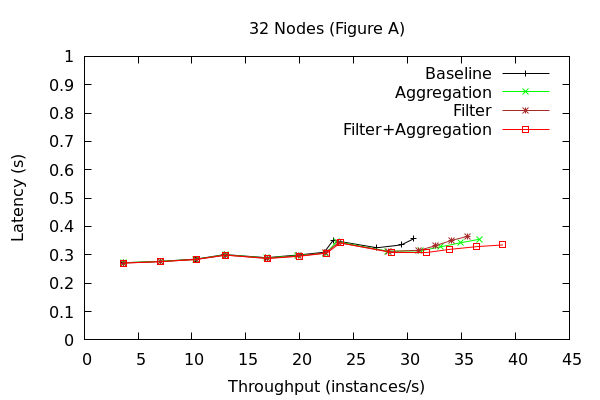
\includegraphics[width=\columnwidth]{figures/32nodes-final.png}
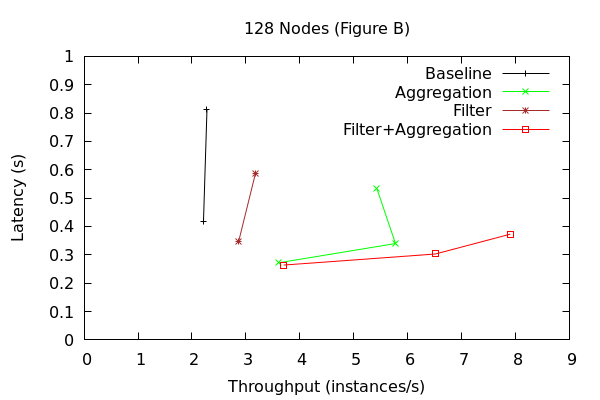
\includegraphics[width=\columnwidth]{figures/128nodes-final.png}
\caption{Overall performance of Baseline, Filter, Aggregation and Filter+Aggregation for 32 and 128 nodes}
\label{fig:overallTendermint}
\end{figure*}

% \begin{figure}[htbp]
% \centering
% 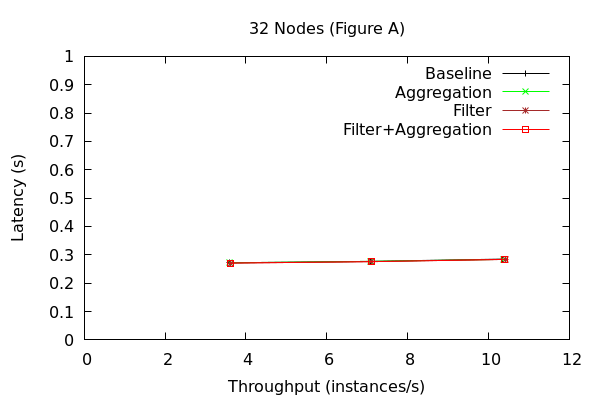
\includegraphics[width=\columnwidth]{figures/32nodes-3points.png}
% \caption{Close up of system performance with 32 nodes in the first three window sizes}
% \label{fig:cdfsW11}
% \end{figure}

In the experiments with 32 nodes,
in configurations with low demand the four setups perform almost equally. When the Baseline reaches saturation (window  $\approx 10$, $\approx 30$ instances per second) we observe that setups Filtering and Aggregation (isolated) allow to further scale, and that the combination of both, Filtering+Aggregation, leads better performance than the isolated cases.  
Table \ref{tab:sturationPoints} shows, for each Semantic Gossip setup, its increase in throughput relative to the Baseline case ('relative' line), up to $ 27 \%$ higher.
%
With 128 nodes the benefit of the proposed mechanisms becomes clearer,
with throughput up to 3.57 $\times$ the Baseline.

To better understand the mechanisms, we take the points with best throughput/latency relation and compute also the average number of received messages to complete an instance, by a process. This is 
shown in Table \ref{tab:msgsRcvdPerInstance}.   We notice that Filtering showed reduction 
of 33 and 43 \% of messages, Aggregation shows important impact with the number of nodes,
with 17 and 71 \% less messages respectively for 32 and 128 nodes.    Also, the mechanisms combined show still better effect than in isolation for both network sizes.


\begin{table}[h!]
\centering
	\begin{tabular}{c c c c c }
	\hline
     Size in     &        &       &       & Filtering+  \\ 
	 Nodes & Baseline   & Filtering    & Aggregation    & Aggregation  \\  \hline
	32  		& 		30.521		&	35.525	&	36.665	&  38.834 \\
	relative   		& 		  1		&	1.16	&	1.20	&  1.27      \\ \hline
	128  		& 		2.213		&	2.865	&	5.773	&  7.902  \\  
	relative   		& 		  1		&	1.29	&	2.60	&  3.57  \\ \hline \\
 
	\end{tabular}
	\caption{Tendermint throughput for different network sizes and  gossip setups, at the best throughput/latency point.}
 \label{tab:sturationPoints}
\end{table}


\fd{following tables to be reviewed due to possible race condition on monitoring variable.}
\begin{table}[h!]
\center
	\begin{tabular}{c c c c c }
	\hline
     Size in     &        &       &       & Filtering+  \\ 
	 Nodes & Baseline   & Filtering     & Aggregation    & Aggregation  \\  \hline
	32  		& 		25.14        &	19.25	&	20.89	&  16.70 \\
 	relative   	& 		  1		     &	0.77	&	0.83	&  0.66      \\ \hline
	128  		& 		109.92	     &	73.91	&	32.03	&  21.35  \\ 
 	relative   	& 		  1		     &	0,67	&	0,29	&  0.19      \\ \hline \\
	\end{tabular}
	\caption{Average of gossip received messages per node, per decided Tendermint instance, at the best throughput/latency point.}
  \label{tab:msgsRcvdPerInstance}
\end{table}

% For each case in Figure~\ref{fig:overallTendermint}, we highlight with a circle
% the point of the highest ratio between average latency and throughput.
% From this point on, increasing client workloads results in small throughput
% increments at the cost of relevant latency increments.


% \rg{In both 32 and 128 we observe that the Baseline requires more than 2f+1 messages to decide on a value., whereas the Filtering, Aggregation and Filtering+Aggregation require less than 2f+1(less or close to none redundancy?).}  \fd{is this correct?  possible? } 



%\rg{Maybe would be better if we just write down the values on the table below? Like "for 32 nodes the percentage was 23.03\% and 23.29\% using filtering and filtering+aggregation, respectively, and for 128...". Just to make it clear, the table represents the percentage of messages that were dropped by the filter at the chosen saturation point(calculated as the ratio between the sum of all messages that all nodes should send and the sum of all filtered messages at all nodes).}

\begin{table}[h!]
\centering
	\begin{tabular}{c c c c c }
	\hline
     Size in     &       &  Filtering+  \\ 
	 Nodes & Filtering    & Aggregation  \\  \hline
	32  		&	23.03\%	&  23.29\% \\
	128  		&	30.09\%	&  29.31\%  \\ \hline \\
	\end{tabular}
	\caption{Percentage of messages filtered out by the semantic filter mechanism at the best throughput/latency point.}
\end{table}

\rg{One thing that maybe is interesting to mention here is that we have 23\% on the execution that were filtered out and we also have a difference of 24\% between the recvMsg/(numNodes*instances) ratios of the Baseline and the Filtering(19.25/25.14 at table III). In other words, as we skip sending 23\% of the messages, the nodes receive 24\% less messages per instance in comparison to the Baseline. Same way, we had 30\% of messages filtered out for 128 nodes and they received 33\% less messages per instance compared to the Baseline.}

\fd{yes ... i am thinking that table II seems a fundamental measure  and maybe other measures just collapse to that...} 


\begin{table}[h!]
\centering
	\begin{tabular}{c c c c c }
	\hline
     Size in     &       &  Filtering+  \\ 
	 Nodes & Aggregation    & Aggregation  \\  \hline
	32  		&	16.77\%	&  13.01\% \\
	128  		&	70.92\%	&  71.76\%  \\ \hline \\
	\end{tabular}
	\caption{Percentage of messages aggregated  at the best throughput/latency point.}
\end{table}
\fd{just reminding.  this is the percentage of messages that were aggregated with others.  it does not measure exactly how many less messages were sent due aggregation.}


\subsection{Latencies}
\label{sec:latency-cdfs}

Window 1 represents the situation where an instance of consensus is proposed only after the previous has been finished, therefore with minimum contention.

For 32 nodes and window 1, we observe in Figure \ref{fig:cdfs}(left) that all setups have the same latency distribution (lines are collapsed).  At the one side this means that the semantic mechanisms did not help to enhance performance.  On the other side, it shows that in a light scenario where the Baseline performs well the semantic mechanisms did not add overhead. 

With 128 nodes, even the window is 1, we notice 
from Figure \ref{fig:overallTendermint}(right), 1st point,
that the Baseline and Filter only configurations do not scale, having latency above the others.  From Figure \ref{fig:cdfs}(right) we observe that
although Filtering is important, Aggregation has the most important impact on latency and their joint use still slightly enhances latency.    Here we notice the importance of Aggregation with growing number of nodes.  As Tendermint uses communication steps with the same types of messages addressed to all participants, the population of messages prone to Aggregation in intermediate nodes, and thus the positive impact of Aggregation, is proportional to the number of nodes.    
%
Interestingly, from Figure \ref{fig:cdfs} we observe that with 128 nodes the Filtering+Aggregation setup shows latency distribution very similar to the reported with 32 nodes, leaving to conclude that this setup reduced communication overhead to be compatible with having $1/4$ of nodes. \fd{really?}   


To detail the behavior with 32 nodes we take from the less performing setup (Baseline) the window with best throughput/latency point (window 11).  With this configuration all setups show similar throughput (see Figure \ref{fig:overallTendermint}(left) 11th point).
The latency distributions of the four setups is depicted in Figure \ref{fig:cdfsW11}.  As the Baseline reaches saturation, latency distributions are slightly better using Semantic Gossip.  Filtering and Aggregation show similar impact, and their combination still reduces latency.   \fd{added what here?}   

An important general observation is that the mechanisms are not delaying instance's decision, even if messages are dropped due to filtering.  On the contrary, latency distributions are consistently better at all percentiles with the mechanisms proposed, showing that sparing redundancy is indeed possible and a good measure.


\begin{figure*}[htbp]
\centering
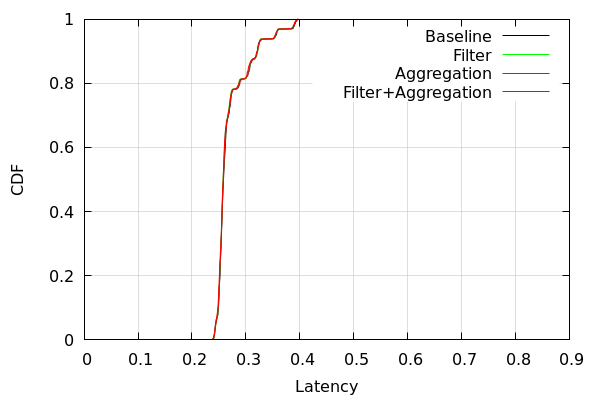
\includegraphics[width=\columnwidth]{figures/w1-32nodes-cdf.png}
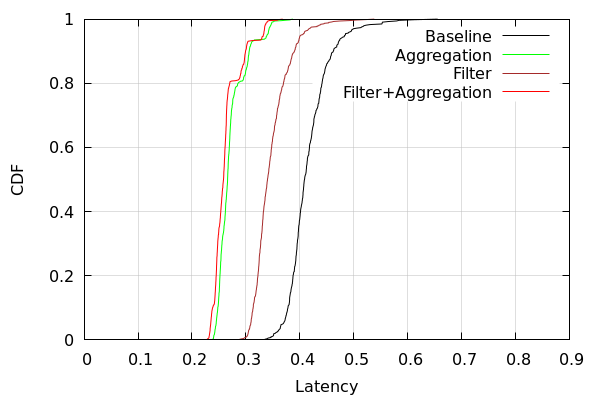
\includegraphics[width=\columnwidth]{figures/128nodes-cdf.png}
\caption{Latency CDFs for Baseline, Filter, Aggregation and Filter+Aggregation, using window 1 for 32 nodes (left) and  128 nodes(right)}
\label{fig:cdfs}
\end{figure*}

\begin{figure}[htbp]
\centering
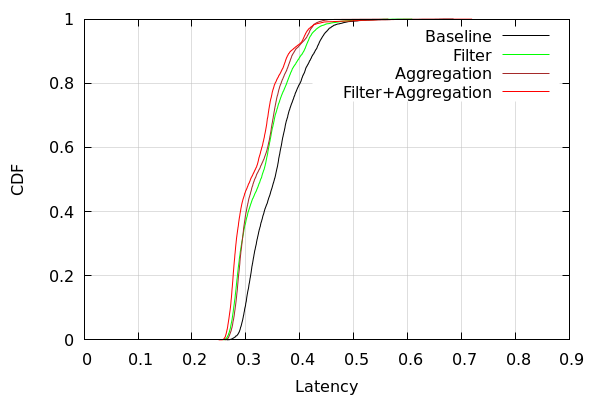
\includegraphics[width=\columnwidth]{figures/w11-32nodes-cdf.png}
\caption{Latency CDf for 32 nodes Window size 11}
\label{fig:cdfsW11}
\end{figure}

\subsection{Resilience}
\label{sec:resilience}

As redundancy is needed to cope with byzantine behavior and since Semantic Gossip is designed to safely eliminate redundancy, we designed experiments to evaluate if and how consensus is affected by byzantine behavior using Semantic Gossip mechanisms in comparison to the Baseline.

Under the assumption that signatures are reliable and since gossip works with signature verification, any attempt to forge or corrupt messages would be detected.   Therefore, we conclude the worst byzantine behavior to harm consensus would be that dishonest nodes remain silent, i.e. they do not collaborate with the consensus protocol.

For 32 and 128 nodes, we incrementally convert honest to byzantine nodes, 5 by 5\%, starting with 0 and going up to 30\%.  Regardless of performance, consensus should show progress in all cases since it supports up to $1/3$ dishonest nodes.  Tables \ref{tab:biz32} and \ref{tab:biz128} show the resulting throughput of the experiment respectively for 32 and 128 nodes.  The first general observation is that all configurations keep progress.   The second is that for 128 nodes all Semantic Gossip configurations performed better than or equivalent to the Baseline.  Thirdly, for 32 nodes, in all configurations the effect of having Filtering+Aggregation slightly enhanced or has equivalent throughput.   For Filtering and Aggregation separated, in most cases performance was equivalent or better than the Baseline.  For 30\% dishonest nodes these setups show performance below the Baseline, indicating that message drop by the mechanisms, added by 30\% of silent nodes, have slightly delayed consensus to be reached.

\begin{table}[h!]
\centering
	\begin{tabular}{c c c c c }
	\hline
     Byzantine     &        &       &       & Filtering+  \\ 
	 Nodes & Baseline   & Filtering    & Aggregation    & Aggregation  \\  \hline
	 0 \%  		    & 		32.177		&	35.069	&	35.219	& 38.297  \\
	 5 \%  		    & 		1.447		&	1.451	&	1.436	& 1.455  \\
	 10 \%  		& 		0.728		&	0.731	&	0.740	& 0.744  \\
	 15 \%  		& 		0.731		&	0.723	&	0.718	& 0.717  \\
	 20 \%  		& 		0.687		&	0.624	&	0.690	& 0.695  \\
	 25 \%  		& 		0.572		&	0.696	&	0.671	& 0.702  \\
	 30 \%  		& 		0.561		&	0.372	&	0.326	& 0.628  \\ \hline \\
	\end{tabular}
	\caption{Tendermint throughput in instances/sec with 32 nodes. 
 Each setup with window of best throughput/latency point with 0 dishonest nodes.   Then converting nodes 5 by 5\% to dishonest.}
 \label{tab:biz32}
\end{table}

\begin{table}[h!]
\centering
	\begin{tabular}{c c c c c }
	\hline
     Byzantine     &        &       &       & Filtering+  \\ 
	 Nodes & Baseline   & Filtering    & Aggregation    & Aggregation  \\  \hline
	 0 \%  		    & 		2.362		&	3.246	&	5.427	& 7.908  \\
	 5 \%  		    & 		0.778		&	0.810	&	0.942	& 1.040  \\
	 10 \%  		& 		0.473		&	0.497	&	0.515	& 0.517  \\
	 15 \%  		& 		0.373		&	0.374	&	0.409	& 0.406  \\
	 20 \%  		& 		0.276		&	0.277	&	0.277	& 0.277  \\
	 25 \%  		& 		0.238		&	0.238	&	0.232	& 0.316  \\
	 30 \%  		& 		0.197		&	0.222	&	0.339	& 0.416  \\ \hline \\
	\end{tabular}
	\caption{Tendermint throughput in instances/sec with 128 nodes. 
 Each setup with window of best throughput/latency point with 0 dishonest nodes.   Then converting nodes 5 by 5\% to dishonest.}
  \label{tab:biz128}
\end{table}



\fd{a análise acima é válida.   acho que podemos seguir pela vazao.
adicionando grafico de thoughput/latencia podemos mostrar que os mecanismos nao prejudicam latencia}


% talvez possamos usar latencia ...

% PARA RESPONDER QUE OS MECANISMOS NAO IMPEDEM A DECISAO,  PODEMOS PEGAR O CASO DE JANELA 1 E VER A LATENCIA PARA DECISOES.   SE A LATENCIA PARA DECISAO FOR MAIOR QUE PARA O BASELINE, EM TESE ALGUMA MENSAGEM ESTA SENDO JOGADA FORA E NAO DEVERIA.   SE TIVER LATENCIA MELHOR, AINDA MELHOR.

% UM ESTUDO ADICIONAL SERIA SUPONDO O SISTEMA EM ALTA UTILIZCAO, COMO IMPACTAM OS BIZANTINOS EM CADA CASO.
% AQUI PEGARIA O CENARIO DE MELHOR THROUGHPUT/LATENCIA EM CADA CASO.
% DAI TERIA QUE PLOTAR O GRAFICO THROUGHPUT/LATENCIA,
% E UMA TABELA DE LATENCIA MEDIA POR INSTANCIA. 

% SENDO CHATO ... ACHO QUE O BOM SERIA TER OS DOIS.
% }

\subsection{Impact of Signature validation with gossip}
\label{sec:signatureImpact}


\begin{table}[h!]
	\begin{tabular}{c c c c c }
	\hline
     Signature     &        &       &       & Filtering+  \\ 
	 Validation & Baseline   & Filtering    & Aggregation    & Aggregation  \\  \hline
	  on  		& 		...		&		&		&   \\
	  off  		& 				&		&		&    \\ \hline \\
	\end{tabular}
	\caption{Saturation point throughput using signature validation, or not, with 
	none (Baseline), Filtering,
	Aggregation and Filtering and Aggregation semantic gossip mechanisms with Tendermint.}
\end{table}

\rg{We have to discuss better the data. }


